% =====================================================================
%  SFLT stochastic energy conservation (Williamson 6, ref 5, 2 days).
%  Exp 3 (amplitude sweep) and Exp 4 (ensemble). Requires \usepackage{graphicx}.
% =====================================================================

\begin{figure}[htbp]
  \centering
  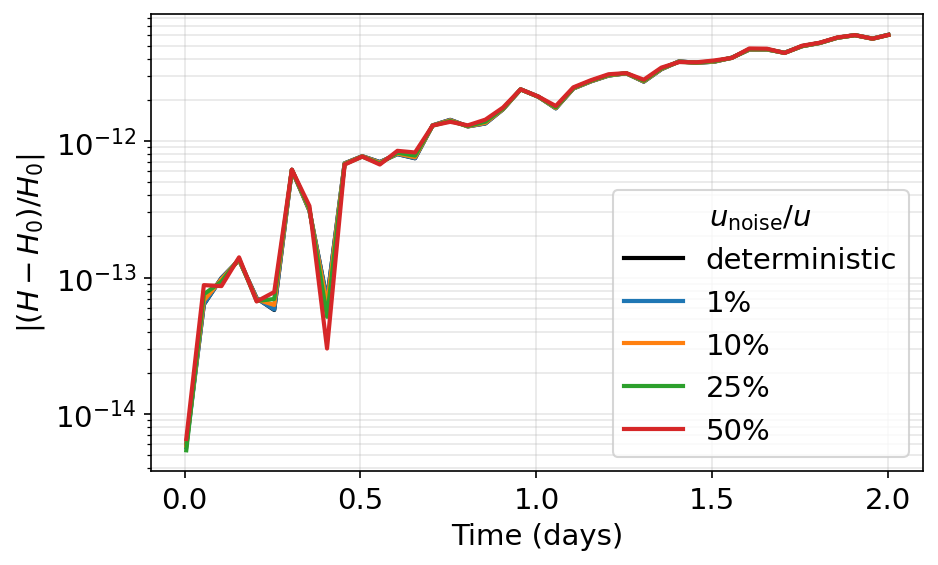
\includegraphics[width=0.8\textwidth]{w6_sflt_amp_sweep.png}
  \caption{Energy conservation of the SFLT stochastic scheme as the noise
    amplitude is varied, for Williamson test case~6, BDM$_2$/DG$_1$, cPG($P_1$),
    refinement level~5, over $2$ days. Each curve is the relative energy drift
    $|(H-H_0)/H_0|$ for a fixed realised noise amplitude
    $u_{\mathrm{noise}}/u \in \{0,\,0.01,\,0.10,\,0.24,\,0.48\}$ (the resolved
    correlation length $\lambda = 6\times10^{6}$\,m is held fixed and only the
    amplitude \texttt{noise\_scale} is changed). All five curves -- including the
    deterministic run -- coincide at the solver/round-off level
    ($\max|(H-H_0)/H_0| = 6.0\times10^{-12}$, identical to three significant
    figures across all amplitudes). The divergence-free Stratonovich transport
    noise therefore adds \emph{no net energy at any forcing strength}: the
    energy-conservation property is structural, not an artefact of weak noise.}
  \label{fig:sflt-amp-sweep}
\end{figure}

\begin{figure}[htbp]
  \centering
  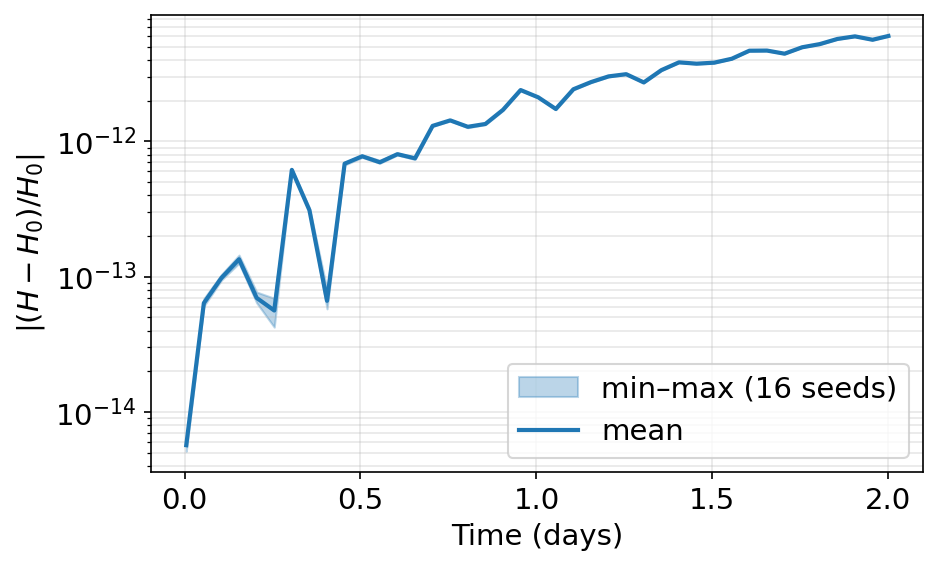
\includegraphics[width=0.8\textwidth]{w6_sflt_ensemble_energy.png}
  \caption{Energy conservation of the SFLT stochastic scheme across an ensemble of
    realisations, for Williamson test case~6 at the physical noise amplitude
    ($u_{\mathrm{noise}}/u \approx 0.10$), refinement level~5, over $2$ days. The
    shaded band is the min--max envelope of the relative energy drift
    $|(H-H_0)/H_0|$ over $16$ random seeds and the solid line is the ensemble
    mean. The entire band lies at the solver/round-off level: the per-seed maxima
    span only $6.00$--$6.05\times10^{-12}$, a spread of $5\times10^{-14}$. Energy
    conservation is thus seed-independent -- no realisation drifts -- confirming
    that the property holds pathwise for the stochastic scheme.}
  \label{fig:sflt-ensemble-energy}
\end{figure}
